% 北京大学博士研究生学位论文开题报告；以 pkuthss 排版。
% 待作者核实：学号、专业、研究方向以及开题日期。
\documentclass[UTF8,openany,oneside]{pkuthss}
\usepackage[backend=biber,style=caspervector,utf8,sorting=none]{biblatex}
\renewcommand*{\bibfont}{\zihao{5}\linespread{1.27}\selectfont}
\setlength{\bibitemsep}{3bp}
\addbibresource{thesis.bib}
\pkuthssinfo{
  cthesisname={博士学位论文开题报告}, ethesisname={Doctoral Research Proposal},
  thesiscover={博士研究生学位论文开题报告},
  ctitle={面向人机共生的注意力驱动定向交互研究},
  etitle={Attention-driven Directional Interaction for Human--Machine Symbiosis},
  cauthor={李景聿}, eauthor={Jingyu Li},
  studentid={2301111877}, school={计算机学院},
  cmajor={计算机系统结构}, emajor={Computer Architecture}, direction={
智能无线网络与移动计算},
  mentorlines={1}, cmentor={许辰人长聘副教授},
  ementor={Prof. Chenren Xu},
  date={二〇二六年九月},
  ckeywords={具身智能，人机共生，注意力定向交互，眼动追踪，脑电意图解码},
  ekeywords={Embodied intelligence, Human--machine symbiosis, Attention-aware interaction, Directional interaction, Eye tracking, EEG},
  degreetype={0}
}
\begin{document}
\frontmatter
\pagestyle{empty}
\maketitle
\cleardoublepage
\pagestyle{plain}
\pagenumbering{Roman}
\begin{cabstract}
随着具身智能与泛在智能物体逐步进入生产和生活环境，人机关系正由人使用单一设备完成离散任务，转向人与多个具身智能体共享物理情境、持续感知彼此状态并动态协作的人机共生。在这一过程中，交互对象、任务进程与环境状态均可能实时变化，用户因而不仅需要“操作设备”，还需要在多个共处对象之间迅速辨认当前目标、自然地表达交互意图，并将指令准确地作用于特定对象。以协同工厂为例，操作人员可能需要在机械臂、移动机器人和智能工位之间连续切换，查看某一对象的状态并随即下达指令，而不应反复退出当前任务以搜索设备。由此，面向多对象的、符合人类空间认知习惯的直观定向交互，成为人机共生时代的新需求。

然而，现有交互方式难以满足这一需求。二维码扫描、设备列表检索和无线配对等方式忽视了指向、朝向与注视中已经包含的空间关注信息；即使用户已明确关注某一对象，仍需在界面中重新查找、确认并连接设备，使物理对象选择、数字身份识别、连接建立与动作执行相互割裂。究其根因，现有系统无法将人的自然注意力直接转化为可靠的对象绑定，只能借助额外的显式步骤恢复交互过程中丢失的注意力信息，因而增加了多对象切换的时间、操作与认知负担。因此，如何捕捉并利用可测量的注意力，在不增加额外操作的前提下准确绑定交互对象，是实现直观定向交互的核心问题。
本文围绕\textbf{如何挖掘、利用人真实注意力并可靠地转化为高效、精准的定向交互}这一问题展开研究。通过对人类注意力信息由浅入深的挖掘和利用，形成\textbf{“所指即所控—所看即所控—所思即所控”}的三种定向交互模式，旨在为未来人机共生提供一个新的交互模式解决方案。具体来说，主要研究工作如下：

（1）针对广泛普及的手机等手持终端，本文提出基于指向的非接触定向交互系统 RetroAR。本文首先发现，手机指向所携带的用户位置和方向信息可由可见光的定向传播特性自然保留。基于此，设计了面向商用手机的可见光定向交互机制：用户以手机闪光灯照射逆反射标签，标签调制反射光并由手机后置摄像头接收，无须检索和连接无线设备。为兼顾数据通信与空间锚定，本文进一步设计动态光标签 ViTag，并结合消息级动态兴趣区、快速凸包检测和自适应时空混合编解码，使系统在手机运动、视角变化和复杂光学背景下稳定读取标签并估计六自由度位姿。系统评估表明，RetroAR 最远可在约 $4\,\mathrm{m}$ 距离和约 $100^\circ$ 视角下工作；用户研究表明，其交互开销相比传统Wi-Fi扫码方案降低50\%，且交互负担更小。RetroAR 验证了光学链路利用“指向”提升定向交互效率的可行性，为“所指即所控”提供系统依据；

（2）针对快速普及的AR眼镜终端，本文提出基于互补红外光学通信的定向交互系统 EchoSight。本文发现，相较于需要主动抬起并对准的手持设备，眼镜方向能够自然贴近用户的观察方向，而红外光束的定向特性可以保留用户注意力指向性，使目标识别与控制一步完成：用户看向目标并做出手势后，眼镜端 SightReader 发射调制红外光，对象端 EchoTag 接收指令并调制反射光，回送身份与状态信息，无须预先注册或建立无线连接。本文进一步设计双路互补光学前端，结合双波段差分信号、对准检测和按需唤醒机制，抑制环境光干扰与非目标响应，实现低时延双向通信。系统评估表明，EchoSight 最远可在约 $5\,\mathrm{m}$ 距离和约 $120^\circ$ 视角下工作；用户研究表明，其交互效率相比二维码扫描和语音控制方案至少提升5倍，且主观负担更低、交互流畅性更好。EchoSight 验证了“视线”比“指向”承载更直观的注意力信息，为“所看即所控”提供系统依据；

（3）针对未来小型化、多模态的新式穿戴设备，本文拟提出利用眼动捕获注意力并结合脑电解码识别意图的定向交互系统 Omnisight。本文首先观察到，用户的眼睛注视朝向和眼镜朝向往往不对齐，且注视方向真正代表了其注意力落点；基于此，设计了由眼动驱动的“物理空间三维鼠标指针”：在AR眼镜上集成基于双目相机的眼动追踪模块，并设计光学云台实现LED波束转向，使光束主动追随用户的真实视线并对准关注目标。与此同时，本文进一步引入基于水凝胶电极的脑电意图识别机制，融合眼动和任务相关脑电信息，区分“看向但不操作”与“主动选择并执行”，以减少因纯注视无交互意图所带来的误操作；Omnisight 的研究旨在探索从“方向近似注意”到“眼动对齐+意图判别”的可行路径，为“所思即所控”提供待验证的系统方案。

\end{cabstract}

\begin{eabstract}
As embodied intelligence and ubiquitous intelligent objects increasingly enter production and everyday environments, the relationship between humans and machines is shifting from the use of a single device for discrete tasks toward human--machine symbiosis, in which people and multiple embodied agents share a physical context, continuously perceive one another's states, and collaborate dynamically. In this setting, interaction targets, task progress, and environmental conditions may all change in real time. Users therefore need not only to operate devices, but also to rapidly identify the intended target among multiple co-located objects, express interaction intent naturally, and direct commands accurately to a specific object. In a collaborative factory, for example, an operator may need to switch continuously among a robotic arm, a mobile robot, and an intelligent workstation, checking the status of one object and immediately issuing a command without repeatedly leaving the current task to search for devices. Intuitive directional interaction that supports multiple objects and conforms to human spatial cognition has thus become a new requirement in the era of human--machine symbiosis.

Existing interaction methods, however, struggle to meet this requirement. QR-code scanning, device-list search, and wireless pairing overlook the spatial focus already conveyed by pointing, orientation, and gaze. Even after users have clearly attended to an object, they must still locate, confirm, and connect to the device again through an interface, separating physical-object selection, digital-identity recognition, connection establishment, and action execution. The fundamental reason is that existing systems cannot directly transform natural human attention into reliable object binding. Instead, they rely on additional explicit steps to recover attention information lost during interaction, thereby increasing the temporal, physical, and cognitive costs of switching among multiple objects. Capturing and exploiting measurable attention to bind an interaction target accurately without additional operations is therefore a central challenge in realizing intuitive directional interaction.

This dissertation investigates \textbf{how to uncover and exploit genuine human attention and reliably transform it into efficient and accurate directional interaction}. By progressively exploring and utilizing human attention, it develops three directional interaction paradigms: \textbf{``point to control, look to control, and intend to control.''} The goal is to provide a new interaction paradigm for future human--machine symbiosis. The main research contributions are as follows.

(1) For widely used handheld devices such as smartphones, this dissertation presents RetroAR, a pointing-based contactless directional interaction system. It first observes that the user's position and orientation conveyed by smartphone pointing can be naturally preserved by the directional propagation of visible light. Based on this observation, it designs a visible-light directional interaction mechanism for commodity smartphones: the user illuminates a retroreflective tag with the smartphone flashlight, while the tag modulates the reflected light and the rear camera receives it, eliminating the need to search for and connect to wireless devices. To support both data communication and spatial anchoring, this dissertation further designs the dynamic optical tag ViTag and combines a message-level dynamic region of interest, fast convex-hull detection, and adaptive spatiotemporal hybrid coding and decoding. These techniques enable the system to read tags reliably and estimate six-degree-of-freedom poses under smartphone motion, viewpoint changes, and complex optical backgrounds. System evaluations show that RetroAR operates at distances of up to approximately $4\,\mathrm{m}$ and viewing angles of up to approximately $100^\circ$. A user study shows that it reduces interaction overhead by 50\% compared with a conventional Wi-Fi and QR-code-based approach, while imposing a lower interaction burden. RetroAR demonstrates the feasibility of using an optical link to improve directional interaction efficiency through pointing, providing a system-level basis for ``point to control.''

(2) For the rapidly growing class of augmented-reality glasses, this dissertation presents EchoSight, a directional interaction system based on complementary infrared optical communication. Compared with handheld devices that must be actively raised and aimed, the orientation of glasses more naturally follows the user's viewing direction, while the directionality of an infrared beam preserves the direction of the user's attention, allowing target identification and control to be completed in a single step. After the user looks at a target and performs a gesture, the glasses-mounted SightReader emits modulated infrared light; the object-mounted EchoTag receives the command, modulates the reflected light, and returns identity and status information without preregistration or a wireless connection. This dissertation further designs a dual-path complementary optical front end and combines dual-band differential signaling, alignment detection, and on-demand wake-up to suppress ambient-light interference and responses from non-target objects, thereby enabling low-latency bidirectional communication. System evaluations show that EchoSight operates at distances of up to approximately $5\,\mathrm{m}$ and viewing angles of up to approximately $120^\circ$. A user study shows that its interaction efficiency is at least five times that of QR-code scanning and voice-control approaches, with a lower subjective workload and greater interaction fluency. EchoSight demonstrates that looking conveys attention more intuitively than pointing, providing a system-level basis for ``look to control.''

(3) For future miniaturized and multimodal wearable devices, this dissertation proposes Omnisight, a directional interaction system that captures attention through eye tracking and recognizes intent through EEG decoding. It first observes that the direction of a user's gaze is often misaligned with the orientation of the glasses and that gaze direction more faithfully indicates where the user's attention is focused. Based on this observation, it designs an eye-tracking-driven ``three-dimensional mouse pointer in physical space.'' A binocular-camera-based eye-tracking module is integrated into AR glasses, and an optical gimbal steers an LED beam so that it actively follows the user's actual line of sight and aligns with the attended target. Meanwhile, this dissertation introduces an EEG-based intent-recognition mechanism using hydrogel electrodes. By combining eye-tracking data with task-related EEG signals, the mechanism distinguishes between ``looking without acting'' and ``actively selecting and executing,'' thereby reducing unintended operations caused by gaze without interaction intent. The Omnisight study aims to explore a feasible path from approximating attention through device orientation to aligning with gaze and discriminating intent, providing a system design to be validated for ``intend to control.''
\end{eabstract}

\tableofcontents
\mainmatter
\chapter{研究背景与挑战}

\section{具身智能与人机共生的发展背景}
人工智能正在由以数字内容处理为主的软件能力，进一步走向能够感知环境、理解任务并作用于物理世界的具身智能。机器人、智能汽车、可穿戴设备、智能家居和新型生产装备持续进入真实场景，使计算不再局限于屏幕之内，而是分布在具有不同形态、位置和功能的物理对象之中。由此，人与机器的关系也开始从“人使用单一工具”转向“人与多类智能体共享环境并协同完成任务”：机器不仅接收预先定义的指令，还会根据环境状态提供信息、提出建议乃至执行动作；人则需要在动态过程中理解机器状态、表达目标并保持必要的监督。

这一变化已成为全球人工智能竞争和产业政策的重要方向。我国《“十四五”机器人产业发展规划》将机器人视为引领产业数字化发展和智能化升级的重要载体，并面向制造、医疗、养老和公共服务等场景推动产品研制与应用拓展\supercite{robot_plan_2021}；2025 年国务院发布《关于深入实施“人工智能+”行动的意见》，进一步提出推动人工智能与经济社会各领域广泛深度融合，加快形成人机协同、跨界融合、共创分享的智能经济和智能社会新形态\supercite{ai_plus_2025}，国家发展改革委随后将人机协作、人机交互和虚实融合概括为智能社会的重要特征，并提出面向人机共生布局新型智能基础设施\supercite{ndrc_symbiosis_2025}。国际上，美国《人工智能行动计划》把自动驾驶、无人机和机器人列为人工智能作用于物理世界的重要形态，提出支持下一代制造并识别机器人制造的供应链挑战\supercite{us_ai_action_plan_2025}；欧盟“Apply AI”战略则把机器人、制造、交通和医疗列为重点领域，通过人工智能工厂、测试验证设施和监管沙盒推动技术由实验室走向市场，同时强调可信、安全和以人为本的应用\supercite{eu_apply_ai_2025}。不同经济体在发展路径和治理方式上各有侧重，但共同表明，人工智能竞争已由模型和算力延伸到智能机器能否进入物理环境、与人协作并形成可持续的生产与服务能力。

政策推动正快速转化为全球产业投入和终端供给。在国内，国家税务总局数据显示，2026 年 1---5 月我国具身智能产业企业销售收入同比增长 22.4\%，机器人本体与整机制造企业销售收入增长 30.1\%，工业企业购进具身智能机器人的金额同比增长 2.3 倍\supercite{china_embodied_tax_2026}；2026 世界机器人大会发布的信息显示，我国人形机器人整机产品已超过 400 款，上半年出货量超过 4 万台，机器人已在多个物流中心参与包裹分拣、在近百家药店承担药品拣选，并开始进入景区讲解、社区巡逻和商业服务等场景\supercite{xinhua_embodied_2026}。在海外，宝马于 2026 年在德国莱比锡工厂启动人形机器人 AEON 的生产试点，使其参与高压电池装配、零部件生产和物料配送；此前美国斯帕坦堡工厂的 Figure 02 已在十个月内参与超过 3 万辆汽车的生产\supercite{bmw_humanoid_2026}。这些中外案例说明，具身智能正由样机展示迁移到真实生产与服务现场，机器也由隔离区域内的固定自动化设备逐步转向能够移动、感知并与工作人员共享作业空间的协作主体。

\begin{figure}[htbp]
  \centering
  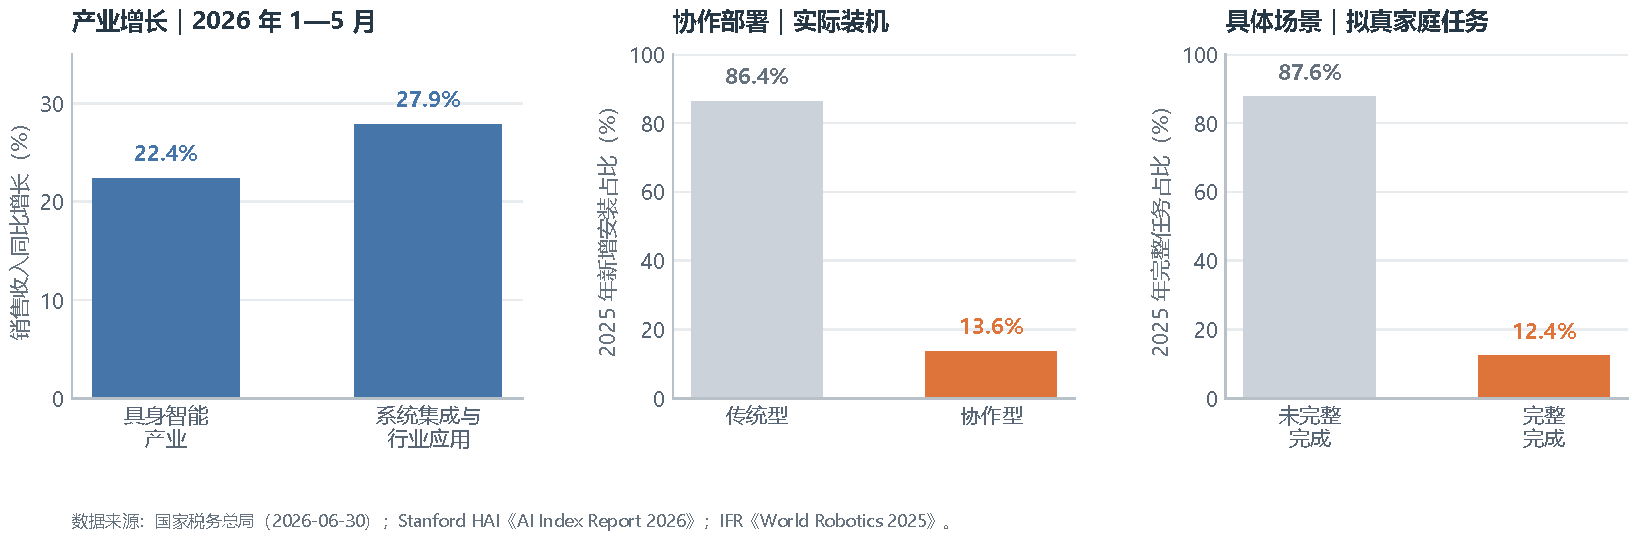
\includegraphics[width=\textwidth]{figs/fig1_1_embodied_ai_landscape.pdf}
  \caption{全球具身智能由政策牵引、产业部署到人机共生挑战的发展态势}
  \label{fig:embodied-ai-development-gap}
\end{figure}

然而，终端数量和展示能力的增长，并不等于人机共生已经成熟。现有案例大多仍集中在物流搬运、部件取放和巡检等边界清晰的任务中，常以少量设备、限定工位或试点项目运行。即使在相对结构化的汽车工厂，宝马仍需先建立统一的数据与接口体系，并在部署过程中增设安全隔离设施、改善厂区 5G 覆盖，再将机器人逐步接入生产流程\supercite{bmw_humanoid_2026}。面向开放环境的行业观察也指出，机器人虽然可以在演示中完成任务，但其速度和可靠性往往尚不足以直接进入工业部署；当不可预测的人进入环境后，机器还必须理解人的语言、手势、姿态和空间指代\supercite{physical_ai_challenge_2026}。

这一现状促使我们思考：\textbf{当具身智能设备已经开始走进工厂、商场、社区和家庭，为什么自然、稳定的人机共生仍未成为普遍现实？} 表面上看，问题表现为机器灵巧性不足、续航有限或模型泛化能力不够；从人机系统的角度看，更深层的原因在于，当前技术主要解决“机器能否完成一个动作”，却尚未充分解决“人如何在复杂现场找到机器、让机器理解自己，并在多个对象之间建立可靠协作关系”。实验室中的一次成功执行通常具有预设目标、已知对象和受控环境，而真实共生场景中的目标、参与者与任务状态会持续变化，两者所需的系统能力并不相同。

首先，现实环境具有开放性和不确定性。物体位置、光照、遮挡和人员活动不断变化，同一指令在不同场景下可能对应不同对象与动作。机器需要把感知结果与物理实体、任务上下文和安全边界联系起来，而不能只复现训练数据中的动作序列。当感知置信度下降或环境发生变化时，系统还要知道何时暂停、请求帮助或把控制权交还给人。这使具身智能的规模化应用不只是模型泛化问题，也是现场状态能否被共同理解的问题。

其次，人机共生环境具有多对象和多主体特征。许多系统仍以“一名用户、一块屏幕、一台预先连接的设备”为基本假设，依靠应用程序、设备名称和菜单层级组织操作。当用户面对多台外观相似的机器人、显示器、传感器或家电时，必须先从网络列表中识别目标，再完成搜索、配对、选择和控制。人在物理空间中已经通过位置、朝向或注视表达了关注对象，数字系统却经常丢失这一信息，导致物理对象、数字身份和交互会话相互分离。

再次，具身智能直接作用于现实世界，交互错误会产生物理后果。系统若选错对象，指令可能被相邻设备执行；若把短暂观察误判为控制意图，又可能触发并非用户所愿的动作。为了规避风险，现有部署常通过隔离区、固定流程和专业人员监督限制机器行为，但这些措施也限制了机器与普通用户自然接触的范围。人机共生因此需要在效率与安全之间取得平衡：既不能让用户为每个简单动作经历冗长配置，也不能把模糊的方向、语音或注视直接解释为高风险命令。

由上述原因可以将人机共生面临的问题归纳为三个系统层面的挑战：一是开放环境下的适应性挑战，机器需要在对象、人员和任务状态持续变化的非结构化现场保持可靠感知与行动，并能在能力边界之外主动求助或交还控制；二是多主体协同挑战，系统需要组织人与多类机器之间的关系，使参与者能够围绕共同目标共享必要的对象、任务和状态信息，而不再依赖“一人一机”的固定配置；三是物理作用下的安全与可信挑战，机器的判断和动作会直接影响现实环境，因而需要控制误操作的后果，并让人能够理解、监督和干预其行为。这三项挑战分别回答机器能否适应现场、多个主体能否形成协作，以及协作能否被安全地接受和使用；其中，如何为人与特定机器建立清晰而低负担的交互关系，是贯穿后两项挑战的基础问题。

综上，具身智能的政策支持、产业投入和终端供给正在全球范围内快速增长，但从可演示、可试点走向可普遍共生，仍存在明显的交互鸿沟。人机共生并不是简单增加机器数量，也不是让机器完全替代人，而是要求人能够自然表达目标，机器能够准确识别对象和意图，双方能够围绕同一任务持续交换状态并处理异常。要跨越这道“最后一公里”，需要从现场空间关系出发重新审视交互入口，使目标发现、身份确认、动作执行与结果反馈围绕同一现实对象连续展开。定向交互由此成为连接具身智能能力与人机共生体验的重要基础。

\section{人机共生环境中的注意力驱动的定向交互}
人机共生环境中的交互具有明确的对象性。用户并不是抽象地向整个环境发出命令，而是在特定时刻希望查看、询问或控制某一个现实对象，例如眼前的机械臂、医疗设备或灯具。当可交互对象由一块屏幕扩展为散布在空间中的大量机器，系统必须先于具体命令回答“用户要与哪一个对象交互”。本文所称的\textbf{定向交互}，即利用用户、交互设备与环境目标之间的空间方向关系，将人的指向映射到特定物理对象，并围绕该对象完成发现、身份确认、命令执行与结果反馈。“定向”既表示人的行为具有空间目标，也要求后续信息仍抵达这个目标，而不是在连接阶段重新退化为对设备列表的搜索。

人的注意力为方向提供了自然线索。人在准备使用物体前，通常会靠近、转头、注视或伸手指向它。不过，心理关注也可以在眼球不转动时发生隐蔽转移，因此注意力并不等同于单一传感器读数，视线只是重要但不完备的观测量\supercite{posner_attention}。本文所称的注意力驱动交互，是指系统利用指向、头向、视线、手部动作和任务上下文估计用户关注的对象，并据此调节目标选择与交互流程；注意力驱动的定向交互则进一步把“用户关注哪里”转化为“系统应与哪一个现实对象建立交互”。其目的不是用眼睛替代鼠标，而是利用人已经自然表达的空间关注，减少重复搜索、命名和配对。

定向交互的发展始于对自然指代行为的数字化。1980 年，麻省理工学院的 ``Put-That-There'' 系统将手势指向与语音结合，由方向回答“哪个对象和位置”，由语音表达动作\supercite{bolt_put_that_there}。1990 年，Jacob 将眼动用于界面目标选择，同时指出眼睛既承担观察任务，又可能被解释为控制命令，从而产生“米达斯接触”问题\supercite{jacobgaze}。进入普适计算阶段，研究重点由操作一台计算机转向管理多设备环境中的注意力。卡内基梅隆大学 2002 年提出 Project Aura，将人的注意力视为普适计算中最稀缺的资源，通过感知用户任务与可用设备减少配置和迁移造成的打断\supercite{project_aura}；随后形成的注意用户界面主张系统根据自己处于注意力前景还是背景决定何时响应\supercite{attentive_user_interfaces}。EyePliances 给出了现实家电实例：电视在无人观看时暂停，AuraLamp 只有在用户看向它时才接受语音命令\supercite{eyepliances}。这些工作确立了“以方向确定目标、以其他线索确认操作”的基本范式。

移动计算、增强现实和可穿戴感知进一步把这一范式带入三维空间。ubiGaze 利用头戴眼动设备把凝视手势附着到真实物体\supercite{ubigaze}，Gaze+Pinch 则以凝视指定目标、以捏合手势确认和操纵，形成“眼睛选择、手部承诺”的多模态分工\supercite{gaze_pinch}。面向物联网，Snap-To-It、Scenariot 和 BLEselect 分别探索借助目标图像、增强现实空间映射和蓝牙到达角选择现实设备\supercite{snaptoit,scenariot,bleselect}。目前研究又开始把眼动、手势、场景视觉和历史行为结合，用注意力帮助情境智能体理解用户任务。2025 年的研究表明，将此前的物体注视轨迹加入视觉语言模型上下文，可以改善模型对当前关注对象和下一步交互对象的判断\supercite{gaze_contextual_ai}。研究重心由瞬时“看向哪里”逐步扩展到持续的对象关联与任务情境。

注意力驱动交互也已进入商业空间计算平台。HoloLens 2 支持头部凝视、眼动凝视和凝视停留，适用于维修人员双手被工具占用且现场噪声不利于语音控制的场景\supercite{hololens_gaze_dwell}；Apple Vision Pro 则把“看向对象并捏合手指”作为 visionOS 的主要间接交互方式\supercite{visionos_interaction}。这些系统证明了注意力方向可以减少光标移动和远距离伸手，但其成熟体验主要建立在平台已知的窗口、三维模型和空间锚点之上。对于未预先建模的机械臂、家电或公共设施，系统仍需完成物体识别、数字身份关联和通信授权，才能把一次“看向”转化为现实操作。
我们不禁思考：\textbf{当设备已经能够测量用户的指向、头向和视线，为什么注意力驱动定向交互仍未成为普遍能力？} 例如，在装有两台同型号机械臂的车间中，眼镜可能测得用户正看向左侧机械臂，相机也识别出“机械臂”类别，但无线网络只返回两个相似的设备名称。系统仍不知道左侧实体对应哪个网络地址，也无法保证启动命令不会发给另一台机器。问题的关键因此不是能否获得一个方向，而是该方向能否被可靠地转化为正确对象、真实意图和一致的信息通道。

由方向线索确定注意目标仍存在较大不确定性。手持设备指向较明确，却要求用户举起并对准；头向便于持续获取，却只能粗略表示视野中心；眼动最接近视觉注意，但会受到标定误差、个体差异、设备滑移和自然扫视影响。日常条件下眼动的准确度和精密度会随用户、目标位置与设备状态明显变化\supercite{everydaygaze}；在三维场景中，角度误差还会随距离放大，同一视线附近可能存在相邻、同类或不同深度的多个物体。将测得的 gaze point 映射为具有语义的 gaze object，本身仍是尚未完全解决的问题\supercite{gaze_to_object_mapping}。此外，用户查看灯具可能只是观察环境，并不意味着希望开灯；人在寻找零件或巡视设备时也会自然扫过大量对象。因此，目标解析不仅要融合指向、头向和视线以判断“关注什么”，还要结合动作与上下文判断当前关注是否足以启动交互。

确定物理目标后，系统仍需将其与唯一的数字身份对齐。相机感知和 Wi-Fi、蓝牙发现分别回答“看见了什么”和“附近有什么设备”，却不能证明视野中的某个实体就是设备列表中的某个地址。在同型号设备密集部署、对象移动或遮挡的场景中，依据外观类别、设备名称或邻近关系建立映射都容易产生歧义。二维码、预注册数据库和空间锚点可以辅助关联，但会引入扫描、部署与维护开销，并可能随设备位置或环境布局变化而失效。物理对象与数字身份之间的断裂，使正确的空间选择仍可能转化为错误的网络连接。

建立连接也不意味着交互已经完成。若每次注视都触发命令，会产生严重误操作；若一律要求长时间停留、语音或手势确认，又会抵消注意力交互的效率。Gaze+Pinch 通过“凝视选择、手势确认”缓解米达斯接触，但眼手配合、目标切换和持续操纵仍缺乏统一规则\supercite{gaze_pinch_challenges}。当用户移动、视线离开或链路短时中断时，系统还需要判断应保持会话、重新验证还是切换目标，并将执行状态和结果返回给用户，否则一次正确选择仍难形成可控的交互过程。

据此，注意力驱动定向交互可归纳为三项相互衔接的核心挑战：\textbf{一是注意目标解析挑战}，需要从带有噪声的多模态方向线索中确定用户关注的现实对象，并判断其是否进入交互状态；\textbf{二是物理--数字身份对齐挑战}，需要把选中的现实实体可靠映射到唯一的设备身份和网络地址；\textbf{三是交互闭环保持挑战}，需要根据操作风险设置确认机制，并在移动、遮挡和目标切换过程中维持命令、状态与反馈的一致性。三者依次回答“面向谁”“连接谁”和“如何持续交互”，共同将人的空间注意转化为可执行、可验证的现实操作。

综上，注意力驱动的定向交互已经由屏幕指向和凝视输入，发展到多设备注意力管理、空间计算与情境智能，但现有成果仍未完全贯通现实对象感知、身份确认和数据传输。要使“所指”“所看”可靠地转化为“所交互”，一方面需要\textbf{定向感知技术}提取注意方向并定位目标，另一方面需要\textbf{定向通信技术}利用空间约束核验目标身份、建立局部链路并返回反馈。光学技术同时具备成像感知、视距传播与波束空间约束能力，为统一注意方向、物理对象和信息通道提供了自然基础。

\section{面向定向交互的通信感知技术发展}
上一节指出，注意力驱动定向交互需要把人的注意方向绑定到物理对象，再将其转化为安全、连续的数字连接，即同时回答“目标在哪里”和“目标是谁”。视觉感知能够恢复对象的位置、类别和姿态，射频通信能够发现节点并维持连接，但二者的空间对象与网络身份并不天然对应。光学信号既可成像又可传输数据，并受光束方向、接收视场和遮挡关系约束，因此为统一注意方向、现实对象与信息通道提供了自然基础。

从实现机制看，光学通信通常采用强度调制与直接检测：发光器件以人眼难以察觉的速度改变光强，光电二极管或相机将接收光转换为电信号并恢复数据。发射光束越窄、接收视场越小，链路覆盖的空间范围越集中，不同方向上的对象也越容易分离。因此，光学用于定向交互的价值不仅在于频谱和速率，更在于通过物理传播范围缩小候选集合，使信息来源与用户面对的空间方向建立直接联系。

光学技术首先被用于\textbf{对象感知与空间锚定}。相机通过外观、二维码或人工标记识别目标，1999 年的 ARToolKit 推动了视觉标记在增强现实注册中的应用\supercite{artoolkit_1999}；2002 年的 FindIT 则使用手持光束唤醒匹配标签，使“照向哪里”直接决定“查询谁”\supercite{findit}。InfoLED、LightAnchors 等系统进一步利用设备指示灯或场景点光源，将数字信息锚定到现实位置\supercite{infoled,lightanchors}。这一路线建立了空间选择能力，但静态标记只能提供预存信息，识别结果仍需借助额外映射才能转化为控制链路。

高效 LED 与光电器件的普及推动技术由对象识别走向\textbf{双向光学通信}。2011 年，IEEE 802.15.7 定义了短距离可见光通信机制，LiFi 随后将单条光链路扩展为支持多用户接入和移动切换的无线网络\supercite{ieee_802_15_7,what_is_lifi}。产业界也开始推动落地：Signify 于 2019 年推出 Trulifi 商用系统，2023 年发布的 IEEE 802.11bb 则将光通信纳入无线局域网标准体系\supercite{signify_trulifi,ieee_802_11bb}。这些里程碑表明，光已由单向信息载体发展为可与现有网络协同的接入媒介。

然而，大量现实对象若采用主动光发射器回传，会带来持续供电、方向对准和硬件成本问题。由此形成的\textbf{无源光学回传}路线，使用主动读写器照射目标，以逆反射材料将入射光送回光源附近，并通过液晶等低功耗调制器在回波上编码身份与状态。Retro-VLC、PassiveVLC 和 TurboBoost 等工作逐步验证并提升了这类双向链路的距离、速率与环境适应性\supercite{retrovlc,passivevlc,turboboost}。当手机或眼镜指向目标时，窄光束先筛选候选对象，近原路返回的信号再确认其身份，使“指向哪个物体”与“数据来自哪个设备”在同一现场链路中得到验证，交互入口也由手持指向逐步走向头向和视线驱动。

方向性既是光学的优势，也是其限制。窄光束和小接收视场能够缩小候选范围、降低误绑定，却容易受到环境光、入射角、人体遮挡和用户移动影响，不适合独立承担长时间连接。射频链路则覆盖广、非视距能力强且基础设施成熟，但难以判断用户关注的是哪个现实对象。这种互补性推动技术路线走向\textbf{光学与射频混合}：定向光链路负责发现目标并读取身份、能力或临时凭据，Wi-Fi、蓝牙等射频网络随后承载可穿越短时遮挡的持续会话。已有 LiFi 与 Wi-Fi 混合网络也验证了局部光接入与广域无线覆盖的协同价值\supercite{hybrid_lifi_wifi}。

相较于单一媒介，混合路线可以在建立射频连接前利用空间方向缩小候选范围，并在选择完成后容忍转头、移动与暂时遮挡；同时，低功耗光标签只需交换身份、授权和少量状态，大数据传输与长期控制可以复用成熟射频设施。其关键不在于简单并列两条链路，而在于保证光学身份与射频地址一致，并合理设计遮挡后的保持、重新验证和目标切换机制，从而将第 1.2 节提出的注意目标解析、物理--数字身份对齐和交互闭环保持落实为完整交互流程。

基于上述脉络，本文以光学通信感知一体化作为注意方向与现实对象之间的入口，并探索光学与射频协同：首先利用手机指向和可见光逆反射实现对象选择与信息回传，继而将入口迁移到智能眼镜和近红外双向链路，进一步结合眼动追踪、可调光束与多模态意图判别，并在目标验证后转入可持续的无线会话，使交互由“所指”走向“所看”与“所欲”。

\chapter{研究现状}

% 本章围绕“如何将人的空间注意可靠地转化为面向特定物体的交互”梳理相关工作。与按通信、视觉和生理信号分别罗列技术不同，本文沿对象选择、身份绑定、意图确认与持续会话这一完整链条组织文献：首先讨论定向光学链路如何把空间方向保留到数据传输中；继而讨论注意力线索如何减少多对象交互中的显式发现与切换；最后讨论眼动与脑电能否进一步区分“看向目标”与“准备操作”。这一组织方式也对应本文从 RetroAR 的“所指即所控”、EchoSight 的“所看即所控”到 Omnisight 的“所思即所控”的递进关系。

\section{定向光学链路}

定向交互首先要求系统回答“当前数据究竟来自哪一个物体”。Wi-Fi、蓝牙等射频技术具有覆盖广和生态成熟的优势，但同一覆盖域中的多个设备共享发现空间，物理对象、网络地址与用户指向之间仍需额外映射。光学无线链路则同时受到发射光束、接收视场和视距关系约束，可以在物理层把通信范围限制到局部方向。因此，光的方向性不仅是信道特征，也能够成为对象选择和身份绑定的交互资源。

早期系统已展示了“以光选物”的基本可行性。Ma et al. 提出的 FindIT Flashlight 使用手持光束唤醒特定标签，使“照向”动作直接参与对象筛选\supercite{findit}；Perli et al. 的 PixNet 通过 LCD--摄像头对构造具有空间分辨能力的链路\supercite{pixnet}。在增强现实场景中，Yang et al. 的 InfoLED 和 Ahuja et al. 的 LightAnchors 进一步复用设备指示灯，将身份信息或虚拟内容锚定到具体光源\supercite{infoled,lightanchors}。这些工作把数字信息附着到空间位置，却主要完成单向发现或显示；对象端主动发光需要额外能量，识别结果也常需再映射到独立的无线控制通道。

\begin{figure}[htbp]
  \centering
  \fbox{\parbox[c][4.0cm][c]{0.86\textwidth}{\centering
  \textbf{图片占位：早期定向光学系统对比}\\[0.6em]
  建议内容：FindIT、PixNet、InfoLED 与 LightAnchors 的收发结构，\\
  对比主动发光、空间分辨、身份承载和后续控制通道。}}
  \caption{早期定向光学链路的代表性系统与功能边界（占位图）}
  \label{fig:early-directional-optical-systems}
\end{figure}

逆反射与光调制为低功耗双向链路提供了另一条路径。Li et al. 提出的 Retro-VLC 将逆反射材料与液晶调制器结合，使标签通过调制入射光回传数据\supercite{retrovlc}；Xu et al. 的 PassiveVLC 通过器件与编码协同设计提高无电池标签的可用性\supercite{passivevlc}；Wu et al. 的 TurboBoosting 则利用多像素液晶和高阶调制提升速率与距离\supercite{turboboost}。这一阶段主要把方向性当作提高空间复用率和降低功耗的信道条件，研究指标集中在误码率、速率、距离和视角，并未系统讨论光束方向与用户所选对象之间的语义对应。

面向密集节点，研究重点又从单链路性能转向空间并发。Xu et al. 的 RetroMUMIMO 挖掘不同液晶标签的脉冲响应差异，在物理层并行解调多个上行并以并发 MAC 降低大规模接入时延\supercite{retromumimo}。2024 年，Ghiasi et al. 同时利用偏振和颜色构造无源可见光 MIMO，使多个液晶子信道的容量接近线性增长\supercite{passivevlc_mimo_2024}；Wang et al. 将事件相机与数字微镜器件结合，并行识别约两千个空间信道，表明事件驱动接收可显著突破传统帧率瓶颈\supercite{selene_2024}。这些进展说明光学空间分集能够提高密集场景下的吞吐与并发度，但“同时读到多个标签”与“只绑定用户此刻关心的标签”仍是两个不同目标。

\begin{figure}[htbp]
  \centering
  \fbox{\parbox[c][4.0cm][c]{0.86\textwidth}{\centering
  \textbf{图片占位：无源光学链路与空间并发}\\[0.6em]
  建议内容：Retro-VLC/PassiveVLC 的单标签链路，及 RetroMUMIMO、\\
  偏振--颜色 MIMO、事件相机+DMD 的多信道设计。}}
  \caption{无源光学链路从单标签通信到空间并发的演进（占位图）}
  \label{fig:passive-optical-concurrency}
\end{figure}

本文的第一项前序工作 RetroAR 正是在这一分界处把通信方向性转化为交互方向性。Li et al. 以商用手机闪光灯和后置摄像头作为读写器，设计动态逆反射标签 ViTag，将手机指向、标签身份读取与六自由度位姿估计放在同一光路中\cite{retroar}。与先做视觉识别再查找 Wi-Fi/BLE 地址的组合方案相比，RetroAR 的关键不在于获得更高通信速率，而在于光束只照亮并读取被指对象，使“物理选择”和“数字身份”同时完成。其系统评估给出最远约 $4\,\mathrm{m}$、最大约 $100^\circ$ 视角的工作范围，用户研究则表明其相较基于 Wi-Fi 的方案显著缩短了多对象任务中的交互时间。

\begin{figure}[htbp]
  \centering
  \fbox{\parbox[c][4.0cm][c]{0.86\textwidth}{\centering
  \textbf{图片占位：无源光学链路与空间并发}\\[0.6em]
  建议内容：Retro-VLC/PassiveVLC 的单标签链路，及 RetroMUMIMO、\\
  偏振--颜色 MIMO、事件相机+DMD 的多信道设计。}}
  \caption{无源光学链路从单标签通信到空间并发的演进（占位图）}
  \label{fig:passive-optical-concurrency}
\end{figure}

第二项前序工作 EchoSight 进一步把移动读写器由手持手机迁移到 AR 眼镜。Li et al. 设计眼镜端 SightReader 与对象端 EchoTag，通过双元件、双波段近红外链路完成指令下行、身份与状态上行，并以对齐检测和按需唤醒抑制非目标响应\supercite{echosight}。该系统不要求预注册或先建立射频连接，达到约 $5\,\mathrm{m}$ 距离和约 $120^\circ$ 视角；其价值在于把“抬起手机并指向”推进为“看向并控制”。不过，EchoSight 的固定光轴实际测量的是眼镜朝向而非眼球视线；当相邻目标密集、头眼分离或视距被遮挡时，目标对齐和会话保持仍会失效。

\begin{figure}[htbp]
  \centering
  \fbox{\parbox[c][4.0cm][c]{0.86\textwidth}{\centering
  \textbf{图片占位：无源光学链路与空间并发}\\[0.6em]
  建议内容：Retro-VLC/PassiveVLC 的单标签链路，及 RetroMUMIMO、\\
  偏振--颜色 MIMO、事件相机+DMD 的多信道设计。}}
  \caption{无源光学链路从单标签通信到空间并发的演进（占位图）}
  \label{fig:passive-optical-concurrency}
\end{figure}

2026 年的研究开始把可见光与射频后向散射置于同一环境物联网架构中，以光完成能量供给、局部发现或控制，再由射频承担非视距连接\supercite{xie_joint_vlc_2026}。这提示定向交互不必把所有阶段都压在单一光路上：光适合确认“是哪一个”，成熟无线链路适合维持“持续可控”。但混合链路也带来新的身份一致性问题，即光学标签与无线地址必须经过可验证绑定，不能把“选中”简单等同于“已授权连接”。

\begin{figure}[htbp]
  \centering
  \fbox{\parbox[c][4.2cm][c]{0.86\textwidth}{\centering
  \textbf{图片占位：定向光学链路的技术演进}\\[0.6em]
  建议内容：主动光标记、无源逆反射、空间并发，\\
  以及 RetroAR 与 EchoSight 从手持指向到佩戴式观察的演进。}}
  \caption{定向光学链路从通信到对象绑定的演进（占位图）}
  \label{fig:directional-optical-links}
\end{figure}

\medskip
\noindent\textbf{本节小结。}现有光学研究已经解决“低功耗地传数据”和“并发地读标签”，RetroAR 与 EchoSight 则进一步把定向光路用于目标绑定，实现从手机指向到眼镜观察的原位交互。方向性仍只是注意力的代理，下一节因而转向用户的指向、头向与注视如何贯穿对象发现、选择和反馈。

\section{注意力驱动的直观交互}

注意力驱动交互试图利用用户已经自然表达的位置、朝向、指向与注视，避免用户在物理对象和数字界面之间重复说明目标。在多对象环境中，一个完整过程至少包括候选对象发现、物理对象与数字身份绑定、动作确认和状态反馈。相关工作可据此分为三类：以视觉或无线信号发现对象，以空间输入选择对象，以及在虚实界面中维持对象状态。它们的差异不只在所用模态，更在于注意线索能够贯穿交互链条的哪一段。

第一类方法通过外部标记、外观或语义模型识别物体。二维码与人工视觉标签能够同时编码身份并提供几何定位，结果明确但要求标记处于视野内；自然特征法避免附加标记，却容易受弱纹理、相似外观、运动模糊和遮挡影响\supercite{wagnertracking}。de Freitas et al. 的 Snap-To-It 允许用户拍摄目标后在云端匹配，接近“拍到即选择”，但依赖预先准备的视觉数据库\supercite{snaptoit}。2024 年，Xu et al. 将几何、语义和视觉语言特征融合进三维场景表示，支持在 AR 中以自然语言搜索现实对象\supercite{spatial_ai_2024}；这类开放词汇方法扩展了可识别对象范围，却不能天然给出设备地址、访问权限和实时状态。

\begin{figure}[htbp]
  \centering
  \fbox{\parbox[c][4.0cm][c]{0.86\textwidth}{\centering
  \textbf{图片占位：现实对象发现方法谱系}\\[0.6em]
  建议内容：人工标记、自然特征、云端图像匹配与开放词汇三维理解，\\
  对比身份明确性、预部署需求、遮挡鲁棒性和设备地址获取能力。}}
  \caption{注意力驱动交互中的现实对象发现方法（占位图）}
  \label{fig:physical-object-discovery}
\end{figure}

第二类方法利用无线测位与空间传感缩小候选范围。Huo et al. 的 Scenariot 将超宽带定位与 SLAM 结合，把智能物体注册进 AR 场景\supercite{scenariot}；Zhang et al. 的 BLEselect 在智能眼镜上利用蓝牙到达角估计感知手势方向，把空间指向与无线身份关联\supercite{bleselect}；Kim et al. 的 IRIS 结合无线指环、手机图像和惯性数据，实现面向智能家居的指向控制\supercite{iris}。这些系统说明射频也能借助阵列或异构传感器获得方向，但通常要求设备预注册、环境建图或维护空间坐标与网络地址的映射，快速切换目标时仍可能出现绑定断点。

第三类工作关注虚拟表示与物理状态的持续一致。Zhu et al. 的 BISHARE 支持手机与头戴式 AR 之间的双向绑定，使手机既被头显感知又可控制虚拟内容\supercite{bishare}；Kaimoto et al. 将虚拟草图转化为实体机器的动作\supercite{sketchedreality}；Zhu et al. 则在 AR 界面与可动玩具之间建立实时映射\supercite{mecharspace}。这类系统将研究从“识别一个对象”推进到“让对象持续可控”，但其重点是已注册对象间的同步，首次接近陌生对象时仍需另行完成发现和授权。

\begin{figure}[htbp]
  \centering
  \fbox{\parbox[c][4.0cm][c]{0.86\textwidth}{\centering
  \textbf{图片占位：对象选择与虚实双向绑定}\\[0.6em]
  建议内容：无线测位/指向缩小候选对象，AR 界面绑定数字身份，\\
  再由无线会话同步物理状态与虚拟反馈。}}
  \caption{从空间对象选择到虚实状态同步的典型流程（占位图）}
  \label{fig:selection-and-bidirectional-binding}
\end{figure}

注意线索能够降低上述过程的显式开销。Pfeuffer et al. 的 gaze+pinch 以凝视定位、捏合确认，确立了 XR 中“快速指向+可靠确认”的常见分工\supercite{gaze_pinch}；其后续总结指出，凝视的速度优势必须与精度、舒适度、反馈和误触发共同权衡\supercite{gaze_pinch_challenges}。Schreiter et al. 对导航、探索与物体操作中的头眼协调进行分析，发现头向与视线的关系随活动而变化，因此不能把头向稳定地视作精确注视\supercite{human_gaze_head_2024}。Wilson et al. 进一步把眼动作为向情境 AI 表达注意的输入，但也强调注意信号需要结合任务上下文解释\supercite{gaze_contextual_ai}。这些近期结果共同表明，“方向更接近目标”并不自动等价于“用户要对目标执行动作”。

从这一视角看，RetroAR、EchoSight 并非孤立的两套光通信系统，而是对注意线索利用程度的两级推进。RetroAR 要求用户主动举起并指向手机，动作显著、意愿较强，代价是占用双手且需要对准\supercite{retroar}；EchoSight 让眼镜朝向自然跟随观察方向，并把身份返回和控制下行维持在同一局部光链路中，减少了设备列表选择和二维码扫描\supercite{echosight}。后者提高了自然度，却也削弱了“主动举机”所隐含的确认作用：用户可能只是阅读或扫视，系统不能仅凭眼镜朝向断定操作意图。

\begin{figure}[htbp]
  \centering
  \fbox{\parbox[c][4.2cm][c]{0.86\textwidth}{\centering
  \textbf{图片占位：注意力驱动的多对象交互链}\\[0.6em]
  建议内容：指向/头向/视线 $\rightarrow$ 候选目标 $\rightarrow$ 数字身份\\
  $\rightarrow$ 意图确认 $\rightarrow$ 会话与反馈，并标出信息断点。}}
  \caption{注意力线索在对象绑定与双向交互中的作用（占位图）}
  \label{fig:attention-interaction-chain}
\end{figure}

\medskip
\noindent\textbf{本节小结。}视觉、测位和虚实同步研究分别改善了对象发现、空间选择与状态保持，RetroAR/EchoSight 的改进是让同一方向线索贯穿“选中—识别—控制”。但 EchoSight 仍以机身朝向近似注视，且注视本身不等于操作；下一节因此讨论用眼动精确定位目标、再以生理证据判别意图的可能性。

\section{基于眼动、脑电信号的意图识别}

眼动是空间注意最直接的可观测线索之一。Jacob et al. 早期即使用视线指定界面元素，并指出眼动交互必须处理“看到即触发”的米达斯接触问题\supercite{jacobgaze}。与手持指向和头向相比，视线转移快、幅度小且不占用双手，适合从密集视野中快速给出候选目标；但它同时承担自然观察功能，系统不能把所有注视都解释为命令。

眼动首先受到测量误差和对象映射误差的限制。Feit et al. 对日常凝视输入的研究表明，准确度与精密度会随用户、屏幕区域和标定状态变化，并直接限制可可靠区分的目标尺寸与间距\supercite{everydaygaze}；Liu et al. 比较现实对象的 gaze-to-object 映射算法，也说明从二维注视点到三维物体的归属并非简单相交测试\supercite{gaze_to_object_mapping}。在 AR 眼镜中，设备滑移、头部运动、深度估计和遮挡还会持续改变眼动坐标、头部坐标与世界坐标之间的标定关系。因此，Omnisight 若以眼动驱动可调光束，首先需要验证的是动态条件下的闭环对齐误差和相邻目标可分性，而不是只报告离线眼动精度。

\begin{figure}[htbp]
  \centering
  \fbox{\parbox[c][4.0cm][c]{0.86\textwidth}{\centering
  \textbf{图片占位：从眼动测量到现实对象映射}\\[0.6em]
  建议内容：眼球坐标、头部坐标与世界坐标的转换链，\\
  标出标定误差、设备滑移、深度歧义和相邻目标混淆。}}
  \caption{眼动驱动现实目标定位中的坐标映射与误差来源（占位图）}
  \label{fig:gaze-to-object-error-chain}
\end{figure}

确认机制用于解决“看见”与“选择”的二义性。凝视停留简单但会牺牲速度并增加视觉负担，凝视加手势、按键或语音则将目标定位与命令确认分开\supercite{gaze_pinch,gaze_pinch_challenges}。这种显式确认可靠且易于理解，应当作为生理意图识别的强基线；只有当双手被占用、必须安静或频繁确认造成明显负担时，引入脑电才具有实际意义。换言之，眼动负责回答“看向哪里”，脑电至多提供“是否存在任务相关心理活动”的附加证据，两者不应被写成可直接读取完整意图。

脑电图（Electroencephalography, EEG）具有无创和时间分辨率高的特点，相关脑机接口大致分为诱发响应与自发活动两类。Farwell et al. 的经典 P300 拼写器利用用户关注低概率刺激时产生的事件相关电位确定目标\supercite{farwellp300}；Gao et al. 总结的 SSVEP 方法则依据注视周期刺激产生的稳态频率响应进行选择\supercite{visualauditorybci}。这两类范式目标明确、可形成较高信息传输率，但通常依赖闪烁刺激、重复试次或时间锁定平均，更适合离散界面选择，而不等价于自然环境中自发产生的操作意图。Abiri et al. 的综述也指出，可穿戴 EEG 仍受低信噪比、非平稳性、个体差异和伪迹影响\supercite{eegbcisurvey}。

\begin{figure}[htbp]
  \centering
  \fbox{\parbox[c][4.0cm][c]{0.86\textwidth}{\centering
  \textbf{图片占位：脑电意图识别范式比较}\\[0.6em]
  建议内容：P300、SSVEP 与自发 EEG 的刺激方式、时间窗口和输出，\\
  对比目标可解释性、响应速度、训练需求与自然交互适用性。}}
  \caption{诱发式与自发式 EEG 意图识别范式（占位图）}
  \label{fig:eeg-intention-paradigms}
\end{figure}

国内研究较早探索了眼动与 EEG 的互补。Wang et al. 在《航空学报》提出决策级融合方法，用眼动的空间与行为特征补充 EEG，对多类人机交互意图的识别优于单模态\supercite{wang_eeg_eye_2021}。Miao et al. 在 2024 年进一步以被动脑机接口建模五类隐式交互意图，说明 EEG 可提供浏览、搜索和处置任务中的区分信息，但其实验仍依赖实验室级 64 导设备与受控界面\supercite{miao_implicit_eeg_2024}。这些工作验证了“额外生理证据可能有益”，也暴露出从离线分类准确率到可穿戴实时交互之间的距离。

2024 年以来，多模态研究开始强调同步建模和自适应融合。Yi et al. 将 P300 与瞳孔收缩、视线响应输入双流多尺度网络，为意识障碍患者提供是/否通信；结果显示多模态系统可补充单一行为量表，但任务仍由强刺激和二选一答案严格约束\supercite{yi_hybrid_bci_2024}。Khanna et al. 在人机交接任务中直接比较 EEG、视线和手部运动，发现视线能够最早且最准确地预测交接意图，而融合主要提升较弱模态\supercite{khanna_handover_2025}。Zhu et al. 于 2026 年进一步以跨模态注意和动态集成融合 EEG、眼动与手势，实现六类交互意图分类\supercite{zhu_multimodal_intent_2026}。这些进展支持按场景动态选择模态，却也提醒系统不能预设 EEG 必然优于低成本行为信号。

对于本文拟开展的 Omnisight，上述文献给出了一条可检验而非预设成功的路线：先以眼动把 EchoSight 的“眼镜大致朝向”推进为“实测视线驱动光束”，完成现实目标与光学身份的精确对齐；再在观看但不操作、主动选择和执行控制等平衡任务中，比较眼动单模态、眼动+显式确认、EEG 单模态和眼动+EEG。评价指标除准确率外，还应包括误触发率、漏检率、决策时延、跨用户泛化、标定成本和佩戴负担。若 EEG 不能在这些端到端指标上稳定优于显式确认，则应保留眼动+低负担确认的退化路径，而不能仅凭离线分类结果宣称“所思即所控”。

\begin{figure}[htbp]
  \centering
  \fbox{\parbox[c][4.2cm][c]{0.86\textwidth}{\centering
  \textbf{图片占位：眼动与 EEG 协同的意图识别框架}\\[0.6em]
  建议内容：眼动给出空间目标，EEG 给出任务相关证据，\\
  置信融合后输出“观察/准备操作”，再决定执行或请求确认。}}
  \caption{眼动定位与脑电辅助判别的分级意图识别框架（占位图）}
  \label{fig:gaze-eeg-intention}
\end{figure}




\chapter{本文工作及当前进展}
\section{总体研究框架与递进假设}
本文以“线索获取—对象绑定—意图确认—会话维持—动作反馈”为统一框架，研究三个逐层深入、但不互相替代的假设。第一，人的手持指向携带可用于选择物理目标的空间信息，方向性光学链路可在同一动作中完成目标发现与局部数据交换；RetroAR 已对该假设提供系统证据。第二，交互入口从手机迁移至眼镜后，用户能在较少手部操作下使用类似观察的动作选中目标，完成原位双向交互；EchoSight 已在相应任务中验证其效率与体验。第三，进一步测量眼动、主动对齐光束，并引入任务相关脑电，可能降低错选与误触发；分层链路可能改善持续会话，但这一假设须由 Omnisight 的完整任务实验检验。

三项工作采用同一分析顺序：\textbf{利用哪种注意力线索、如何绑定物理对象、如何通信与反馈、有哪些实验依据、留下什么问题}。RetroAR 和 EchoSight 的既有结果分别支持前两项假设，不直接证明第三项在神经信号、延迟或连接性上的收益。尤其不能把“眼镜朝向”混同于“实测眼动”，也不能把“看向”混同于“想操作”。

\section{RetroAR：从空间指向到目标绑定（已完成）}
\subsection{注意力线索与系统设计}
RetroAR 面向移动增强现实中的非接触定向交互\parencite{retroar}。用户举起手机，闪光灯照向目标端的逆反射标签 ViTag；标签用液晶矩阵调制反射光，手机后置摄像头接收返回信息。光束方向与摄像头视场共同约束候选对象，把“指向目标”和“发现目标”结合起来，无须先从无线列表查找对象。需要准确指出：系统利用的是手机空间指向这一\textbf{间接注意力代理}，没有测量用户实际视线。

为了让指向真正成为可用的交互入口，系统不仅要检测标签，还要在手机运动、视角变化和背景干扰下保持读取。动态兴趣区减少重复搜索的计算开销，几何检测帮助定位标签，自适应时空混合解码恢复信息，并协同支持六自由度位姿估计。这些设计共同服务于“选得中、读得出、跟得稳”，而非彼此独立的算法堆叠。

\subsection{已有证据与通向下一阶段的局限}
原论文报告最远约 $4\,\mathrm{m}$、最大约 $100^\circ$ 的工作范围，六自由度位姿估计的平移误差低至约 $1\,\mathrm{cm}$、旋转误差低至约 $4.7^\circ$；在所设非接触控制任务中，交互时间相较 Wi-Fi 对照方案减少两倍以上\parencite{retroar}。这些结果表明光的方向性能够保留用户的空间选择信息，并减少特定任务中的识别/连接开销，但不可脱离原实验条件外推。

RetroAR 的代价是用户必须拿起、移动并维持手机对准。手机光束可能与人想看的位置接近，但仍由手部动作间接表达关注。这一局限提出下一阶段问题：\textbf{如果方向可以选中对象，能否不用手持设备来表达这个方向？}

\section{EchoSight：从手持指向到佩戴式观察（已完成）}
\subsection{注意力线索与系统设计}
EchoSight 将交互入口从手机迁移至智能眼镜\parencite{echosight}。眼镜端 SightReader 与目标端 EchoTag 构成双向光学链路；双元件近红外光学设计及对齐检测利用空间方向抑制非目标响应，使用户在观察目标时获取信息并发送控制数据。系统延续了 RetroAR 的“方向性可选择目标”思想，但把指向动作尽量嵌入日常佩戴和观察，而不再要求每次举起手机。

局部光学链路把对象身份和信息交换放在同一个现场通道中，减少预注册与额外网络连接需求；双向能力又使用户在识别后能直接操控实体对象，而不止于读取标签。这是从“选择线索”向“原位交互”深入的关键。不过，EchoSight 的方向线索主要来自眼镜前端光路与用户观察方向的近似关系，\textbf{并非实测眼动追踪}。

\subsection{已有证据与通向下一阶段的局限}
CHI 2025 论文报告最远约 $5\,\mathrm{m}$ 的房间尺度通信和最大约 $120^\circ$ 的观察视角；其 12 名参与者的用户研究，在所设任务及对照条件下，显示相对二维码扫描、语音控制至少五倍的交互延迟降低，并报告更低的主观负担\parencite{echosight}。这些证据支持佩戴式、原位双向交互的效率与体验优势，但不能据此证明眼镜始终准确知道用户眼球注视点。

进一步的局限有三点：眼镜机身朝向和眼球实际视线可能偏离，固定光路仍可能迫使人调整姿态；用户看见某物可能只是观察而非操作；遮挡或转头可中断全光会话。由此引出第三阶段的核心问题：\textbf{能否让系统跟随真实视线，并可靠地区分“看见”与“想操作”？}

\section{Omnisight：从观察线索到视线对齐与意图判别（拟开展）}
Omnisight 是拟开展的毕业研究，以下模块均作为待实现、待验证的设计，不作为已经测得的系统结论。其总体思路是把先前依赖设备方向的目标选择推进为实测眼动驱动的对齐，再把目标定位与意图确认分开，并用不同链路分别承担选择和持续会话。

\subsection{实测眼动驱动的目标对齐}
首先，拟在眼镜端获取眼球视线并驱动可调光学发射单元，使光束方向尽可能跟随关注目标。系统需要标定眼动坐标、眼镜/头部姿态和光束坐标之间的变换，并在不同目标距离、相邻目标间距、头部运动和遮挡下测量对齐误差。将与固定光路方案比较目标选错率、对齐时延、功耗和佩戴负担，判定主动调节是否值得增加硬件复杂度。如果眼动置信度低，系统应暂缓执行并请求确认，而非把不确定目标当作正确目标。

\subsection{眼动与脑电的意图判别}
其次，拟在“看向但不操作”“主动选择目标”“执行确认”等可重复任务中，同步采集眼动与凝胶电极脑电，构建与实际交互动作相联系的标签。眼动用于定位候选对象；脑电仅被视为可能有增量价值的判别证据，需要处理眼动和肌电伪迹、个体差异与跨场景迁移。研究将比较仅眼动、仅脑电、融合方法以及眼动加显式确认的基线，报告误触发率、漏检率、精确率、召回率和决策时延，而不是只报告离线分类准确率。

脑电是否成为可用交互通道，取决于其增益是否覆盖采集、佩戴和计算成本。如果在控制眼动信息后，EEG 对误触发的改善不稳定或不足，系统将采用眼动加显式确认的备选路线，并把这一边界作为研究结论。

\subsection{定向选择与持续会话的分层链路}
最后，拟用下行定向光完成目标发现与身份确认，再经授权把该物理目标绑定到蓝牙设备身份；蓝牙承担上行反馈和后续持续会话。光负责“是哪一个”，蓝牙负责“如何保持交互”，两者之间需设计目标标识、状态机、超时、切换和重绑定机制，避免选中物体与实际控制设备不一致。实验应分别测试静止、转头、遮挡和移动场景中的绑定错误率、会话恢复时间、端到端延迟及能耗。混合设计的价值须以这些指标证明，不能假设蓝牙天然免配对或零开销。

目前的工作描述以研究问题、总体架构及关键器件方向为主；眼镜原型、脑电同步、融合模型和混合链路协议仍待实现或系统评估。最终交付应包括可复现实验原型、清晰的对照与消融、完整任务用户研究，以及对收益和成本的实证边界。

\section{综合比较：注意力利用如何逐级深入}
表\ref{tab:progression}把三项工作放在同一交互链上，区分已验证能力与拟检验能力。第一条递进路径是\textbf{注意力线索越来越贴近人}：手机方向、眼镜方向、实测视线与任务相关生理证据。第二条路径是\textbf{系统利用越来越接近行动决策}：先选中物体，再支持原位双向交互，最后检验是否真的应执行控制。第三条路径是\textbf{人对设备的适应负担逐步减少}：从举机对准，经过眼镜近似对齐，走向光束主动追随视线。

\begin{table}[htbp]
\centering\zihao{5}
\caption{三项工作对注意力利用的递进关系}
\label{tab:progression}
\begin{tabular}{p{2.0cm}p{2.8cm}p{4.7cm}p{3.7cm}}
\hline
系统 & 主要线索 & 已解决或拟解决的环节 & 尚需面对的边界 \\
\hline
RetroAR & 手持设备指向 & 已验证目标绑定与局部读取 & 持机、手动对准 \\
EchoSight & 眼镜光路近似观察 & 已验证原位双向交互 & 视线偏离、意图二义性 \\
Omnisight（拟） & 眼动与脑电 & 拟验证主动对齐、意图判别 & 增益、误触发、佩戴与链路开销 \\
\hline
\end{tabular}
\end{table}

统一框架并不意味着对所有场景都自动有效。只有空间线索能够可靠约束候选目标、实体与设备身份可验证绑定、意图确认的收益超过其成本时，注意力驱动交互才能真正改善体验。因此，最终评价必须比较完整任务中的时间、正确性与负担，而不是把三篇论文中不同实验条件下的单项数值简单排列。

\chapter{研究计划}
\section{论文提纲}
计划中最终完成的学位论文将分为五章。全文以“注意力如何转化为可靠、可执行的定向交互”为主线，按照注意力由间接到直接、系统能力由目标选择到意图判别的顺序展开三项工作。各章内容安排如下：

第一章绪论：提出人机共生环境中的多对象定向交互问题，分析从目标发现、对象绑定、意图确认到会话维持与动作反馈的关键挑战；在此基础上，建立注意力外化、注意力对齐和意图判别逐级深入的研究框架，并概述本文的研究内容与主要贡献。

第二章基于手机指向的移动增强现实定向交互系统：介绍 RetroAR 的设计、实现与评估。该章研究如何将用户的手机指向转化为可计算的空间关注，利用可见光逆反射标签在同一光学链路中完成目标发现、身份读取与空间定位，并通过动态兴趣区、时空混合解码和六自由度位姿估计实现“所指即所控”。

第三章基于眼镜观察方向的原位双向交互系统：介绍 EchoSight 的设计、实现与评估。该章将定向交互入口由手持设备迁移至智能眼镜，研究双元件、双波段近红外光路和对齐检测机制，实现在无需预注册和额外无线配对条件下的原位双向交互，并分析由“所指即所控”向“所看即所控”推进所带来的自然性收益及其能力边界。

第四章眼、脑联合的注意力驱动意图交互系统：介绍 Omnisight 的设计、实现与评估。该章在 EchoSight 的基础上引入实测眼动，驱动可调光学发射单元主动对齐目标；进一步利用脑电辅助区分日常观看与主动操作，并研究定向光学选择通道与蓝牙持续会话通道之间的可验证绑定。该章将通过固定与可调光束对照、多模态消融和完整任务用户研究，检验“所思即所控”的可行性、实际收益与适用边界。

第五章总结与展望：总结手机指向、眼镜观察方向以及眼动与脑电三类注意力在对象选择、意图确认和持续交互中的递进关系，归纳注意力驱动定向交互的设计原则与适用条件，并讨论其在多对象人机共生环境中的后续研究方向。

\section{时间进度安排}
在前述三项工作中，RetroAR 与 EchoSight 的系统设计、原型实现和实验评估已经完成；Omnisight 的总体架构与实验问题已经明确，但眼镜原型、眼动与脑电同步、融合模型、混合链路协议及系统评估仍待完成。围绕 Omnisight 研究和学位论文撰写，计划设置以下四个时间节点：
\begin{enumerate}
  \item 在 2026 年 10 月 31 日以前，完成眼动追踪、可调光学发射和脑电采集模块的接入，建立统一时间戳与基础标定流程，完成眼动、头部姿态和光束坐标之间的转换，并记录系统同步误差与初步对齐误差。
  \item 在 2026 年 12 月 30 日以前，完成观看与主动操作任务范式、脑电预处理和离线分类基线，明确跨用户验证方法；同时完成光学目标标识与蓝牙设备身份的可验证绑定，以及目标切换、会话超时、重绑定和恢复机制，形成可执行的端到端 Omnisight 原型。
  \item 在 2027 年 2 月 31 日以前，完成固定与可调光束对照、眼动与脑电多模态消融及完整任务用户研究，系统评估目标错选率、误触发率、漏检率、决策与端到端时延、会话恢复时间、功耗和用户负担；在复核实验结果与系统边界的基础上，完成 Omnisight 研究论文的撰写与投稿。
  \item 在 2027 年 3 月 31 日以前，整合 RetroAR、EchoSight 与 Omnisight 三项工作，完成学位论文的撰写、修改和答辩准备。
\end{enumerate}

\printbibliography[heading=bibintoc,title={参考文献}]
\end{document}
